\chapter{Interface Utilisateur}
\section{Gestion des données}
\subsection{Hyper-X}
Nous avons choisi hyperX pour host la machine virtuelle de Rocky Linux, car disponible par défaut sur les machines windows et a de très bonne performance. Ceci est de plus que une architecture de test donc ce choix n'est pas réelement important.
\subsection{Rocky Linux}
Le choix de Rocky Linux Minimal en tant que base pour le déploiement de conteneurs Docker s'avère judicieux pour plusieurs raisons. En optant pour cette distribution Linux, qui est issue d'une fourche de CentOS et conçue dans un esprit de stabilité et de fiabilité, les utilisateurs peuvent bénéficier d'un environnement solide et sécurisé pour exécuter leurs applications conteneurisées. La version "Minimal" de Rocky Linux offre une empreinte réduite, ce qui permet d'allouer davantage de ressources aux conteneurs eux-mêmes plutôt qu'au système d'exploitation sous-jacent.
\subsection{Docker}
Dans la quête d'une maintenance et d'un déploiement plus simples et efficaces des serveurs,nous avons choisi Docker qui se distingue comme la solution idéale. Grâce à sa capacité à encapsuler des applications et leurs dépendances dans des conteneurs isolés, Docker nous garantit une gestion harmonieuse des versions et des configurations.
\subsection{Mosquitto}
C'est là que Mosquitto entre en jeu en tant que courtier MQTT (Message Queuing Telemetry Transport) open source, offrant une infrastructure pour la transmission de données entre les appareils.
\subsection{MangoDB}
Nous utiliserons ensuite MangoDB, en tant que système de gestion de base car il offre une flexibilité sans pareille pour modéliser des données variées.
\subsection{Node-Red}
Nous avons choisi node-red pour être le subscriber au serveur Mosquitto, et pour gérer les données reçus et les stocker dans la base de données MangoDB. Ce choix est peut être pas le plus efficace, mais il est le plus simple à mettre en place et à maintenir.
\subsection{Docker Compose}
On a choisi d'écrire nos configuration de serveur sous la forme d'un docker compose pour simplifié le déploiement.

\lstinputlisting[language=YAML,caption={Orchestration des containeurs}]{../rocky-linux/docker/docker-compose.yml}


\subsection{utilisateur}
 l'utilisateur a la possibilité d'effectuer différentes actions comme définir à quelle luminosité les phares de son vélo s'activeront. 
 \begin{center}
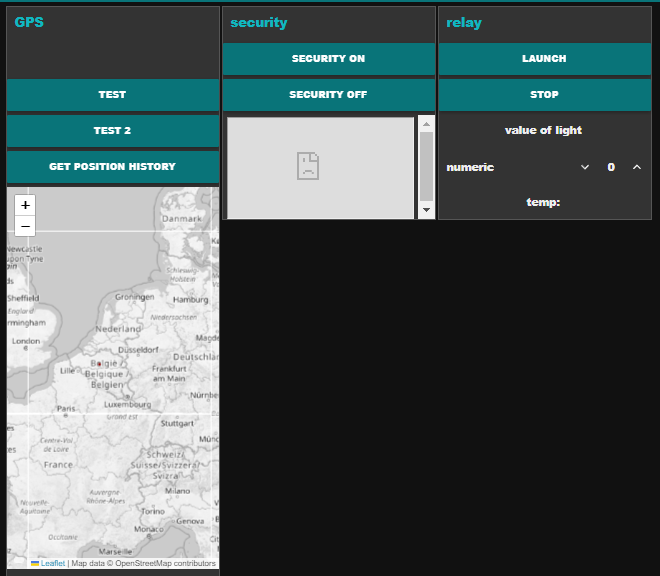
\includegraphics{Rapport/media/images/info.png}{\centering}
\end{center}
\subsection{administrateur}
 l'interface administrateur donne quelques infos utiles que preuve récupérer l'utilisateur pour obtenir une aide à distance.

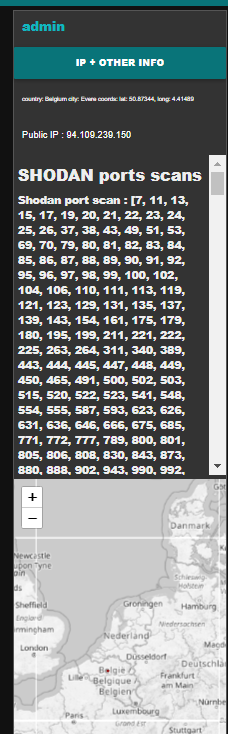
\includegraphics{Rapport/media/images/admin.png}